\documentclass[12pt,a4paper]{article}
\usepackage[utf8]{inputenc}
\usepackage{amsmath}
\usepackage{amsfonts}
\usepackage{amssymb}
\usepackage{graphicx}
\usepackage{pgfplots}
\pgfplotsset{compat=1.18}
\usepackage[left=2cm,right=2cm,top=2cm,bottom=2cm]{geometry}
\usepackage{enumitem}

\begin{document}

\begin{center}
  \textbf{\Large KUIS ke 1}\\[0.5cm]
  \textbf{\large Waktu : 100 menit}
\end{center}
\vspace{0.5cm}

\begin{enumerate}
  \item Dapatkan himpunan penyelesaian dari pertidaksamaan berikut :
        \[ \frac{x^2 - 16}{(x - 1)^2} < 0 \]

  \item Dapatkan himpunan penyelesaian dari nilai mutlak berikut :
        \[ |3x + 1| = 6x \]

  \item Tentukan persamaan garis yang melalui titik(8,2) dan tegak lurus dengan garis $10y + 3x = -2$

  \item Diketahui $f(x) = x - 1$ dan $g(x) = |x^2 - 4|$
        \begin{enumerate}[label=\alph*.]
          \item Dapatkan $g \circ f(x)$
          \item Tentukan domain dan range $g \circ f(x)$
        \end{enumerate}

  \item Diketahui $f(x) = (x - 2)^3 + 1$
        \begin{enumerate}[label=\alph*.]
          \item Dapatkah invers fungsinya
          \item Sketsalah grafiknya
        \end{enumerate}
\end{enumerate}

\vspace{0.5cm}
\begin{center}
  \textbf{\Large PEMBAHASAN}
\end{center}


\begin{enumerate}
  \item Agar pecahan bernilai negatif, karena penyebut $(x-1)^2 > 0$ untuk setiap $x \neq 1$, maka pembilang haruslah negatif:
        \[ x^2 - 16 < 0 \]
        Faktorkan persamaan di atas:
        \[ (x - 4)(x + 4) < 0 \]
        Akar-akarnya adalah $x = 4$ dan $x = -4$.
        Berdasarkan garis bilangan, nilai $x$ yang memenuhi adalah $-4 < x < 4$.
        Namun, karena penyebut tidak boleh nol, maka $x - 1 \neq 0 \implies x \neq 1$.
        Jadi, Himpunan Penyelesaiannya (HP) adalah:
        \[ \text{HP} = \{ x \mid -4 < x < 1 \text{ atau } 1 < x < 4, x \in \mathbb{R} \} \]

  \item Karena ruas kiri berupa nilai mutlak, maka ruas kanan harus tak negatif.
        Syarat: $6x \geq 0 \implies x \geq 0$.

        Kasus 1: $3x + 1 \geq 0$ atau $x \geq -\frac{1}{3}$
        \begin{align*}
          3x + 1 = 6x \implies
          1 = 3x \implies
          x = \frac{1}{3}
        \end{align*}
        (Memenuhi syarat $x \geq 0$)

        Kasus 2: $3x + 1 < 0$ atau $x < -\frac{1}{3}$
        \begin{align*}
          -(3x + 1)  = 6x           \implies
          -3x - 1    = 6x           \implies
          -1         = 9x           \implies
          x          = -\frac{1}{9}
        \end{align*}
        (Tidak memenuhi syarat $x \geq 0$)

        Jadi, Himpunan Penyelesaiannya (HP) adalah:
        \[ \text{HP} = \left\{ \frac{1}{3} \right\} \]

  \item Pertama, cari gradien dari garis $10y + 3x = -2$.
        \begin{align*}
          10y & = -3x - 2                      \\
          y   & = -\frac{3}{10}x - \frac{1}{5}
        \end{align*}
        Gradien garis tersebut adalah $m_1 = -\frac{3}{10}$.
        Karena garis yang dicari tegak lurus, maka perkalian gradiennya adalah $-1$.
        \begin{align*}
          m_1 \cdot m_2            = -1                             \implies
          -\frac{3}{10} \cdot m_2 = -1 \implies m_2 = \frac{10}{3}
        \end{align*}
        Persamaan garis yang melalui titik $(x_1, y_1) = (8, 2)$ dengan gradien $m_2 = \frac{10}{3}$:
        \begin{align*}
          y - y_1       & = m_2(x - x_1)        \\
          y - 2         & = \frac{10}{3}(x - 8) \\
          3(y - 2)      & = 10(x - 8)           \\
          3y - 6        & = 10x - 80            \\
          10x - 3y - 74 & = 0
        \end{align*}

  \item
        \begin{enumerate}[label=\alph*.]
          \item Mencari $g \circ f(x)$:
                \begin{align*}
                  (g \circ f)(x) & = g(f(x))            \\
                                 & = g(x - 1)           \\
                                 & = |(x - 1)^2 - 4|    \\
                                 & = |x^2 - 2x + 1 - 4| \\
                                 & = |x^2 - 2x - 3|
                \end{align*}

          \item Domain dan Range $(g \circ f)(x)$:

                \textbf{Domain:}
                Berdasarkan definisi fungsi komposisi, domain dari $(g \circ f)(x)$ adalah:
                \[ D_{g \circ f} = \{ x \in D_f \mid f(x) \in D_g \} \]
                Diketahui $f(x) = x - 1$ adalah fungsi linear, maka $D_f = \mathbb{R}$.
                Fungsi $g(u) = |u^2 - 4|$ adalah fungsi nilai mutlak dari polinomial, maka $D_g = \mathbb{R}$.
                Sehingga:
                \[ D_{g \circ f} = \{ x \in \mathbb{R} \mid (x - 1) \in \mathbb{R} \} = \mathbb{R} \]
                Jadi, domain $(g \circ f)(x)$ adalah $\mathbb{R}$ atau $(-\infty, \infty)$.

                \textbf{Range:}
                Berdasarkan definisi, range dari $(g \circ f)(x)$ adalah hasil peta dari $g(u)$ untuk semua $u \in R_f$:
                \[ R_{g \circ f} = \{ y \mid y = g(u), u \in R_f \} \]
                Pertama, kita tentukan range fungsi $f(x) = x - 1$ pada $x \in D_f$. Karena fungsinya berupa garis lurus untuk semua $x \in \mathbb{R}$, maka rentangnya adalah $R_f = \mathbb{R}$.
                Kemudian, kita cari hasil pemetaan $u \in R_f$ (atau $u \in \mathbb{R}$) ke dalam $g(u) = |u^2 - 4|$.
                Untuk $u \in \mathbb{R}$, nilai minimum dari fungsi kuadrat $u^2 - 4$ adalah $-4$, sehingga rentangnya adalah $[-4, \infty)$.
                Karena fungsi $g(u)$ memutlakkan nilai tersebut, maka daerah hasil $[-4, \infty)$ akan termutlakkan menjadi tidak negatif. Seluruh nilai negatif dari $[-4, 0)$ menjadi $(0, 4]$, dan nilai positif $[0, \infty)$ tetap $[0, \infty)$. Gabungannya akan menutup seluruh bilangan tak negatif.
                Jadi rentang (range) dari $(g \circ f)(x)$ adalah:
                \[ R_{g \circ f} = [0, \infty) \]
        \end{enumerate}

  \item
        \begin{enumerate}[label=\alph*.]
          \item Mencari invers fungsi $f(x)$:
                Misalkan $y = f(x)$
                \begin{align*}
                  y               & = (x - 2)^3 + 1       \\
                  y - 1           & = (x - 2)^3           \\
                  \sqrt[3]{y - 1} & = x - 2               \\
                  x               & = \sqrt[3]{y - 1} + 2
                \end{align*}
                Jadi, invers fungsinya adalah:
                \[ f^{-1}(x) = \sqrt[3]{x - 1} + 2 \]

          \item Sketsa grafik $f(x) = (x - 2)^3 + 1$ dan $f^{-1}(x) = \sqrt[3]{x - 1} + 2$:
                Titik penting pada $f(x)$ adalah: titik potong sumbu-y $(0, -7)$, titik potong sumbu-x $(1, 0)$, dan titik belok $(2, 1)$.
                Berdasarkan konsep invers, grafik $f^{-1}(x)$ adalah hasil pencerminan grafik $f(x)$ terhadap garis $y = x$.
                Oleh karena itu, titik-titik penting pada $f^{-1}(x)$ merupakan kebalikan dari titik penting $f(x)$, yaitu: $(-7, 0)$, $(0, 1)$, dan $(1, 2)$.

                \begin{center}
                  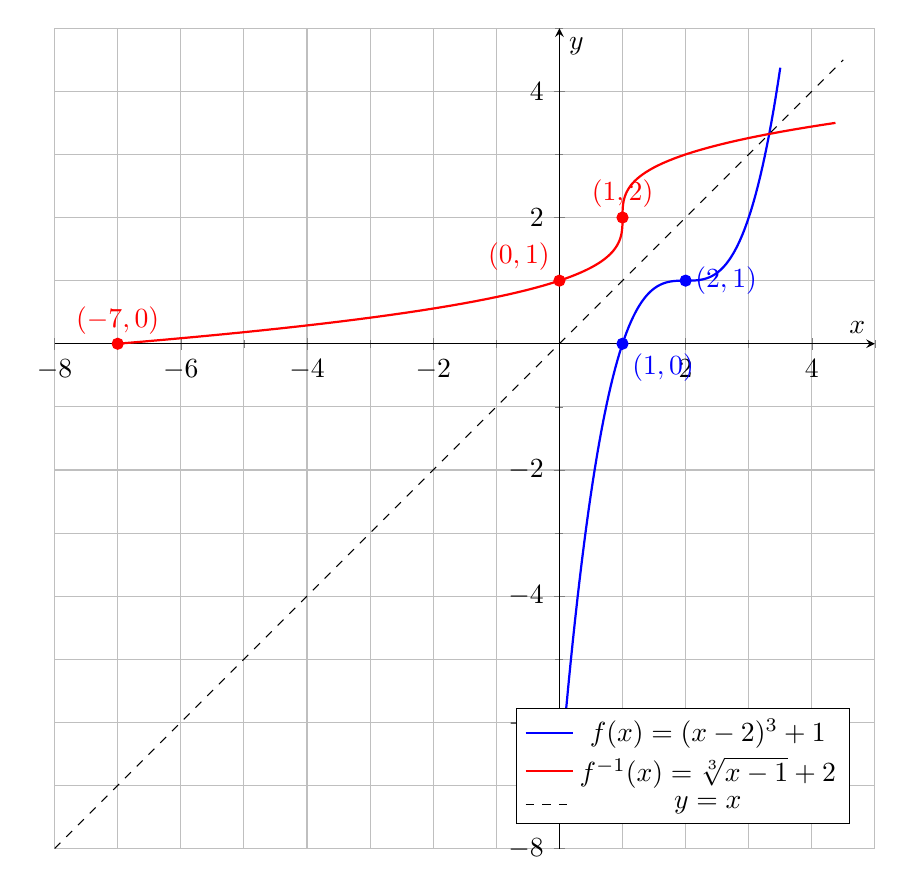
\begin{tikzpicture}
                    \begin{axis}[
                        axis lines = middle,
                        xlabel = $x$,
                        ylabel = $y$,
                        ymin=-8, ymax=5,
                        xmin=-8, xmax=5,
                        grid=both,
                        minor tick num=1,
                        width=12cm,
                        height=12cm,
                        samples=100,
                        legend pos=south east
                      ]
                      % Grafik f(x)
                      \addplot[domain=0:3.5, thick, blue] {(x-2)^3 + 1};
                      \addlegendentry{$f(x) = (x-2)^3+1$}

                      % Grafik f^{-1}(x) dengan metode parametrik (menukar x dan y dari f(x))
                      \addplot[domain=0:3.5, thick, red] ({(x-2)^3 + 1}, {x});
                      \addlegendentry{$f^{-1}(x) = \sqrt[3]{x-1}+2$}

                      % Garis pantul y = x
                      \addplot[domain=-8:4.5, dashed, black] {x};
                      \addlegendentry{$y = x$}

                      % Titik penting f(x)
                      \addplot[mark=*, blue] coordinates {(0, -7)} node[right]{$(0, -7)$};
                      \addplot[mark=*, blue] coordinates {(1, 0)} node[below right]{$(1, 0)$};
                      \addplot[mark=*, blue] coordinates {(2, 1)} node[right]{$(2, 1)$};

                      % Titik penting f^{-1}(x)
                      \addplot[mark=*, red] coordinates {(-7, 0)} node[above]{$(-7, 0)$};
                      \addplot[mark=*, red] coordinates {(0, 1)} node[above left]{$(0, 1)$};
                      \addplot[mark=*, red] coordinates {(1, 2)} node[above]{$(1, 2)$};
                    \end{axis}
                  \end{tikzpicture}
                \end{center}
        \end{enumerate}

\end{enumerate}

\end{document}
